% --------------------------------------------------------------
% This is all preamble stuff that you don't have to worry about.
% Head down to where it says "Start here"
% --------------------------------------------------------------
 
\documentclass[12pt]{article}
 
\usepackage[margin=1in]{geometry} 
\usepackage{amsmath,amsthm,amssymb}
\usepackage{graphicx}
\usepackage{tikz}
\usetikzlibrary{arrows}
\newcommand{\N}{\mathbb{N}}
\newcommand{\Z}{\mathbb{Z}}
 
\newenvironment{theorem}[2][Theorem]{\begin{trivlist}
\item[\hskip \labelsep {\bfseries #1}\hskip \labelsep {\bfseries #2.}]}{\end{trivlist}}
\newenvironment{lemma}[2][Lemma]{\begin{trivlist}
\item[\hskip \labelsep {\bfseries #1}\hskip \labelsep {\bfseries #2.}]}{\end{trivlist}}
\newenvironment{exercise}[2][Exercise]{\begin{trivlist}
\item[\hskip \labelsep {\bfseries #1}\hskip \labelsep {\bfseries #2.}]}{\end{trivlist}}
\newenvironment{problem}[2][Problem]{\begin{trivlist}
\item[\hskip \labelsep {\bfseries #1}\hskip \labelsep {\bfseries #2.}]}{\end{trivlist}}
\newenvironment{question}[2][Question]{\begin{trivlist}
\item[\hskip \labelsep {\bfseries #1}\hskip \labelsep {\bfseries #2.}]}{\end{trivlist}}
\newenvironment{corollary}[2][Corollary]{\begin{trivlist}
\item[\hskip \labelsep {\bfseries #1}\hskip \labelsep {\bfseries #2.}]}{\end{trivlist}}
\newenvironment{solution}
  {\begin{proof}[Solution]\renewcommand{\qedsymbol}{}}
  {\end{proof}}

\usepackage{listings}
\usepackage{color}

\definecolor{mygreen}{rgb}{0,0.6,0}
\definecolor{mygray}{rgb}{0.5,0.5,0.5}
\definecolor{mymauve}{rgb}{0.58,0,0.82}

\lstset{ %
  backgroundcolor=\color{white},   % choose the background color; you must add \usepackage{color} or \usepackage{xcolor}
  basicstyle=\footnotesize,        % the size of the fonts that are used for the code
  breakatwhitespace=false,         % sets if automatic breaks should only happen at whitespace
  breaklines=true,                 % sets automatic line breaking
  captionpos=b,                    % sets the caption-position to bottom
  commentstyle=\color{mygreen},    % comment style
  deletekeywords={...},            % if you want to delete keywords from the given language
  escapeinside={\%*}{*)},          % if you want to add LaTeX within your code
  extendedchars=true,              % lets you use non-ASCII characters; for 8-bits encodings only, does not work with UTF-8
  frame=single,                    % adds a frame around the code
  keepspaces=true,                 % keeps spaces in text, useful for keeping indentation of code (possibly needs columns=flexible)
  keywordstyle=\color{blue},       % keyword style
  language=Python,                 % the language of the code
  morekeywords={*,...},            % if you want to add more keywords to the set
  numbers=left,                    % where to put the line-numbers; possible values are (none, left, right)
  numbersep=5pt,                   % how far the line-numbers are from the code
  numberstyle=\tiny\color{mygray}, % the style that is used for the line-numbers
  rulecolor=\color{black},         % if not set, the frame-color may be changed on line-breaks within not-black text (e.g. comments (green here))
  showspaces=false,                % show spaces everywhere adding particular underscores; it overrides 'showstringspaces'
  showstringspaces=false,          % underline spaces within strings only
  showtabs=false,                  % show tabs within strings adding particular underscores
  stepnumber=1,                    % the step between two line-numbers. If it's 1, each line will be numbered
  stringstyle=\color{mymauve},     % string literal style
  tabsize=2,                       % sets default tabsize to 2 spaces
  title=\lstname                   % show the filename of files included with \lstinputlisting; also try caption instead of title
}

\begin{document}


 
% --------------------------------------------------------------
%                         Start here
% --------------------------------------------------------------
 
\title{Homework 3}%replace X with the appropriate number
\author{Maksim Levental\\ %replace with your name
MAP 4102} %if necessary, replace with your course title
 
\maketitle
 
\begin{problem}{1a} %You can use theorem, exercise, problem, or question here.  Modify x.yz to be whatever number you are proving
Prove or disprove the Markov chain

\begin{center}
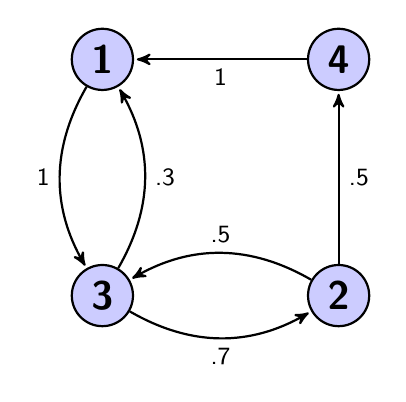
\begin{tikzpicture}[->,>=stealth',shorten >=1pt,auto,node distance=3cm,
  thick,main node/.style={circle,fill=blue!20,draw,font=\sffamily\Large\bfseries}]

  \node[main node] (1) {1};
  \node[main node] (2) [below of=1] {3};
  \node[main node] (3) [right of=1] {4};
  \node[main node] (4) [below of=3] {2};

  \path[every node/.style={font=\sffamily\small}]
    (3) edge node {1} (1)
    (1) edge [bend right] node[left] {1} (2)
    (2) edge [bend right] node[right] {.3} (1)
        edge [bend right] node[below] {.7} (4)
    (4) edge node[right] {.5} (3)
        edge [bend right] node[above] {.5} (2);
\end{tikzpicture}

\end{center}
converges to a limiting distribution.
\end{problem}
 
\begin{solution}

The Markov of chain does not converge. It is irreducible (to wit $4 \rightarrow 1 \rightarrow 3 \rightarrow 2 \rightarrow 4$) and the period of state $1$ is 2 (to wit there are only 3 unique pathes from $1$ to $1$: $1\rightarrow 3 \rightarrow 1$, $1\rightarrow 3\rightarrow 2\rightarrow 3 \rightarrow 1$, $1\rightarrow 3 \rightarrow 2 \rightarrow 4\rightarrow 1$ and they have lengths which are multiples of 2) so the chain oscillates between 2 configurations. To wit 
$$\begin{pmatrix}
0.481 & 0.518 & & \\
0.481 & 0.518 & & \\
& & 0.740 & 0.259 \\
& & 0.740 & 0.259 
\end{pmatrix}
$$

\begin{center}and\end{center}

$$\begin{pmatrix}
 0.740 & 0.259& & \\
 0.740 & 0.259& & \\
& &0.481 & 0.518 \\
& &0.481 & 0.518 
\end{pmatrix}
$$



\end{solution}

\ \\ \\

\begin{problem}{1b} %You can use theorem, exercise, problem, or question here.  Modify x.yz to be whatever number you are proving
Prove or disprove the Markov chain


\begin{center}
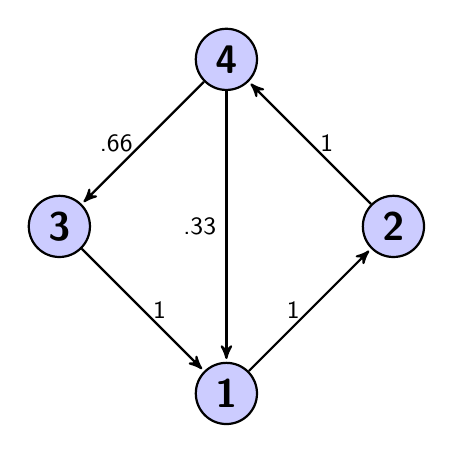
\begin{tikzpicture}[->,>=stealth',shorten >=1pt,auto,node distance=3cm,
  thick,main node/.style={circle,fill=blue!20,draw,font=\sffamily\Large\bfseries}]

  \node[main node] (4) {4};
  \node[main node] (3) [below left of=4] {3};
  \node[main node] (2) [below right of=4] {2};
  \node[main node] (1) [below left of=2] {1};

  \path[every node/.style={font=\sffamily\small}]
    (4) edge node[left] {.33} (1)
        edge node[left] {.66} (3)
    (1) edge node[left] {1} (2)
    (2) edge node[right] {1} (4)
    (3) edge node[right] {1} (1);
\end{tikzpicture}
\end{center}
converges to a limiting distribution.

\end{problem}
 
\begin{solution} 

The Markov chain does converge to a limiting distribution. The chain is obviously irreducible so by Thm. 1.14 it has a unique stationary distribution. The period of state $2$ is one because $2 \rightarrow 4 \rightarrow 1 \rightarrow 2$ is a valid traversal with length $3$ and so is $2 \rightarrow 4 \rightarrow 3 \rightarrow 1 \rightarrow 2$ with length $4$ ($gcd(3,4)=1$). So the chain is aperiodic and by Thm. 1.19 it converges to its stationary distribution. To wit

$$ p^n(x,y) = \frac{1}{11}(3,3,2,3)$$

\end{solution}



\begin{problem}{1c} %You can use theorem, exercise, problem, or question here.  Modify x.yz to be whatever number you are proving
Prove or disprove the Markov chain


\begin{center}
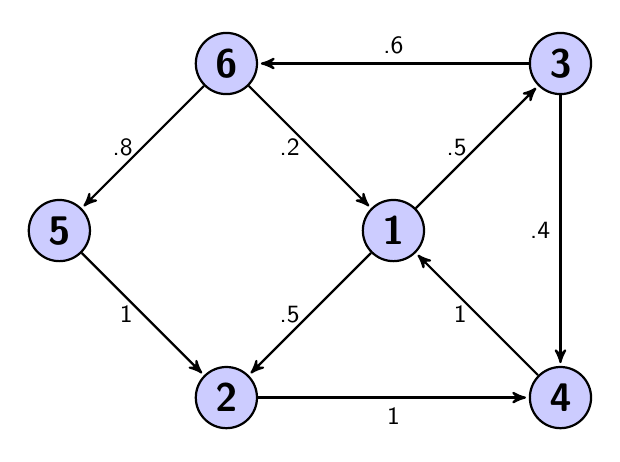
\begin{tikzpicture}[->,>=stealth',shorten >=1pt,auto,node distance=3cm,
  thick,main node/.style={circle,fill=blue!20,draw,font=\sffamily\Large\bfseries}]
  
  \node[main node] (1) {1};
  \node[main node] (2) [below left of=1] {2};
  \node[main node] (3) [above right of=1] {3};
  \node[main node] (4) [below right of=1] {4};
  \node[main node] (6) [above left of=1] {6};
  \node[main node] (5) [below left of=6] {5};

  \path[every node/.style={font=\sffamily\small}]
    (1) edge node[left] {.5} (2)
        edge node[left] {.5} (3)
    (2) edge node[below] {1} (4)
    (3) edge node[left] {.4} (4)
        edge node[above] {.6} (6)
    (4) edge node[left] {1} (1)
    (5) edge node[left] {1} (2)
    (6) edge node[left] {.2} (1)
        edge node[left] {.8} (5);
\end{tikzpicture}

\end{center}
converges to a limiting distribution.
\end{problem}
 
\begin{solution} 

The Markov chain does not converge to a limiting distribution. The chain is irreducible:

$$ 6\rightarrow 5\rightarrow 2\rightarrow 4\rightarrow 1\rightarrow 3\rightarrow 6.$$
The period of of state $5$ is 6; the only path from $5$ to $5$ without repetition is of length $6$:

$$ 5 \rightarrow 2\rightarrow 4\rightarrow 1\rightarrow 3\rightarrow 6\rightarrow 5.$$
So the period of the Markov chain is three (the period of state $1$ is three) and hence the chain oscillates between 3 ``configurations''. We omit the three $6\times6$ matrices.

\end{solution}


\begin{problem}{2}

Compute the stationary distribution for

$$
\setcounter{MaxMatrixCols}{20}
\begin{pmatrix}
0 & & & &.5 & & & & & & & & & &.5 \\
1 & & & & & & & & & & & & & & \\
 &1 & & & & & & & & & & & & & \\
 & &1 & & & & & & & & & & & & \\
 & & &1 & & & & & & & & & & & \\
 & & & &1 & & & & & & & & & & \\
 & & & & &1 & & & & & & & & & \\
 & & & & & &1 & & & & & & & & \\
 & & & & & & &1 & & & & & & & \\
 & & & & & & & &1 & & & & & & \\
 & & & & & & & & &1 & & & & & \\
 & & & & & & & & & &1 & & & & \\
 & & & & & & & & & & &1 & & & \\
 & & & & & & & & & & & &1 & & \\
 & & & & & & & & & & & & &1 &0 \\  
\end{pmatrix}
$$

\end{problem}
\begin{solution}
By the relation $\boldsymbol{\pi} P = \boldsymbol{\pi}$ the Markov chain induces a system of linear equations:


\begin{align*}
\frac{1}{2}\pi_4 + \frac{1}{2}\pi_{14} &= \pi_0 \\
\pi_0 &= \pi_1 \\
\pi_1 &= \pi_2 \\
\vdots &= \vdots \\
\pi_{13} & = \pi_{14}
\end{align*}
So $\pi_{14}$ is the only free variable. Solving for $\pi_{14}$ subject to the condition that $\frac{1}{2}\pi_{14} + \frac{1}{2}\pi_{14} = \pi_{14}$ and $\sum_{i=0}^{14}\pi_i = 1$ yields the stationary distribution $\pi_y =\frac{1}{15} $ for all $y$.

\end{solution}
% --------------------------------------------------------------
%     You don't have to mess with anything below this line.
% --------------------------------------------------------------

 
\begin{problem}{3a} %You can use theorem, exercise, problem, or question here.  Modify x.yz to be whatever number you are proving
Find the transition probability matrix representation for the Markov chain

\begin{center}
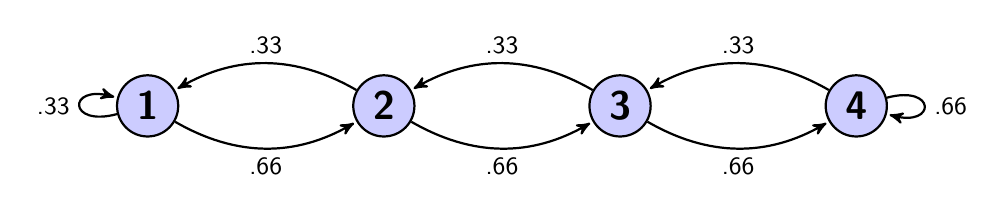
\begin{tikzpicture}[->,>=stealth',shorten >=1pt,auto,node distance=3cm,
  thick,main node/.style={circle,fill=blue!20,draw,font=\sffamily\Large\bfseries}]

  \node[main node] (1) {1};
  \node[main node] (2) [right of=1] {2};
  \node[main node] (3) [right of=2] {3};
  \node[main node] (4) [right of=3] {4};

  \path[every node/.style={font=\sffamily\small}]
    (1) edge [bend right] node[below] {.66} (2)
        edge [loop left]  node[left]  {.33} (1)
    (2) edge [bend right] node[below] {.66} (3)
        edge [bend right] node[above] {.33} (1)
    (3) edge [bend right] node[below] {.66} (4)
        edge [bend right] node[above] {.33} (2)
    (4) edge [bend right] node[above] {.33} (3)
        edge [loop right]  node[right]  {.66} (4);
        %% (3) edge node {1} (1)
    %% (1) edge [bend right] node[left] {1} (2)
    %% (2) edge [bend right] node[right] {.3} (1)
    %%     edge [bend right] node[below] {.7} (4)
    %% (4) edge node[right] {.5} (3)
    %%     edge [bend right] node[above] {.5} (2);
\end{tikzpicture}

\end{center}
\end{problem}
\ \\
\begin{solution}
The transition matrix is straightforward:
$$
\begin{pmatrix}
.33 & .66 & & \\
.33&  &.66 & \\
&.33 & &.66 \\
& & .33 & .66 
\end{pmatrix}
$$
\end{solution}
\begin{problem}{3b}
Find the limiting amount of time the chain spends at each site.
\end{problem}
\begin{solution}
The chain is irreducible (all states clearly communicate), aperiodic ( $p(0,0)=.33 >0$ ), and has a stationary distribution (because it is irreducible and finite). So by Thm. 1.22 the asymptotic frequency of state $y$ is the $y$-th entry in the stationary distribution. The stationary distribution is
$$ \pi = \frac{1}{15}(1,2,4,8) $$ 
So the chain spends $\frac{1}{15}$ of its time in state 1, $\frac{2}{15}$ of its time in state 2, $\frac{4}{15}$ of its time in state 3, and $\frac{8}{15}$ of its time in state 4.
\end{solution}
\end{document}



\begin{align*}
\sum_{i=1}^{k+1}i & = \left(\sum_{i=1}^{k}i\right) +(k+1)\\ 
& = \frac{k(k+1)}{2}+k+1 & (\text{by inductive hypothesis})\\
& = \frac{k(k+1)+2(k+1)}{2}\\
& = \frac{(k+1)(k+2)}{2}\\
& = \frac{(k+1)((k+1)+1)}{2}.
\end{align*}


\end{solution}
$$
\begin{alignat*}{2}
\rho_{AA} &= \rho_{BA} \cdot p(A,B) + \rho_{CA} \cdot p(A,C) = \rho_{BA} \cdot \frac{1}{2} + \rho_{CA} \cdot \frac{1}{2} & \\
\rho_{CA} &= \rho_{AA'} \cdot p(C,A) + \rho_{BA} \cdot p(C,B) = 1 \cdot  \frac{1}{2} + \rho_{BA} \cdot \frac{1}{2} & \\
\rho_{BA} &= \rho_{DA} \cdot p(B,D) = 0 \cdot 1 = 0
\end{alignat*}
Note that $\rho_{AA}$ and $\rho_{AA'}$ are different; $\rho_{AA}$ is the probability of hitting $A$ for some time $n\geq 1$ and $\rho_{AA'}$ is the probability of hitting $A$ for sometime $n \geq i$ given that $X_i = A$. Hence
\begin{alignat*}{2}
\rho_{CA} &= 1 \cdot \frac{1}{2} + 0 \cdot \frac{1}{2} = \frac{1}{2} \\
\rho_{AA} &= 0 \cdot \frac{1}{2} + \frac{1}{2} \cdot \frac{1}{2} = \frac{1}{4} \\
\end{alignat*}
